\appendix{Представление графического материала}

Графический материал, выполненный на отдельных листах,
изображен на рисунках А.1--А.\arabic{числоПлакатов}.

\setcounter{числоПлакатов}{0}
\renewcommand{\thefigure}{А.\arabic{figure}} % шаблон номера для плакатов

\begin{landscape}

\begin{плакат}
    
\includegraphics[width=0.82\linewidth]{posters/1.eps}
    \заголовок{Сведения о ВКРБ}
    \label{pl1:image}
\end{плакат}

\begin{плакат}
    
\includegraphics[width=0.82\linewidth]{posters/2.eps}
    \заголовок{Цель и задачи разработки}
    \label{pl2:image}
\end{плакат}

\begin{плакат}
    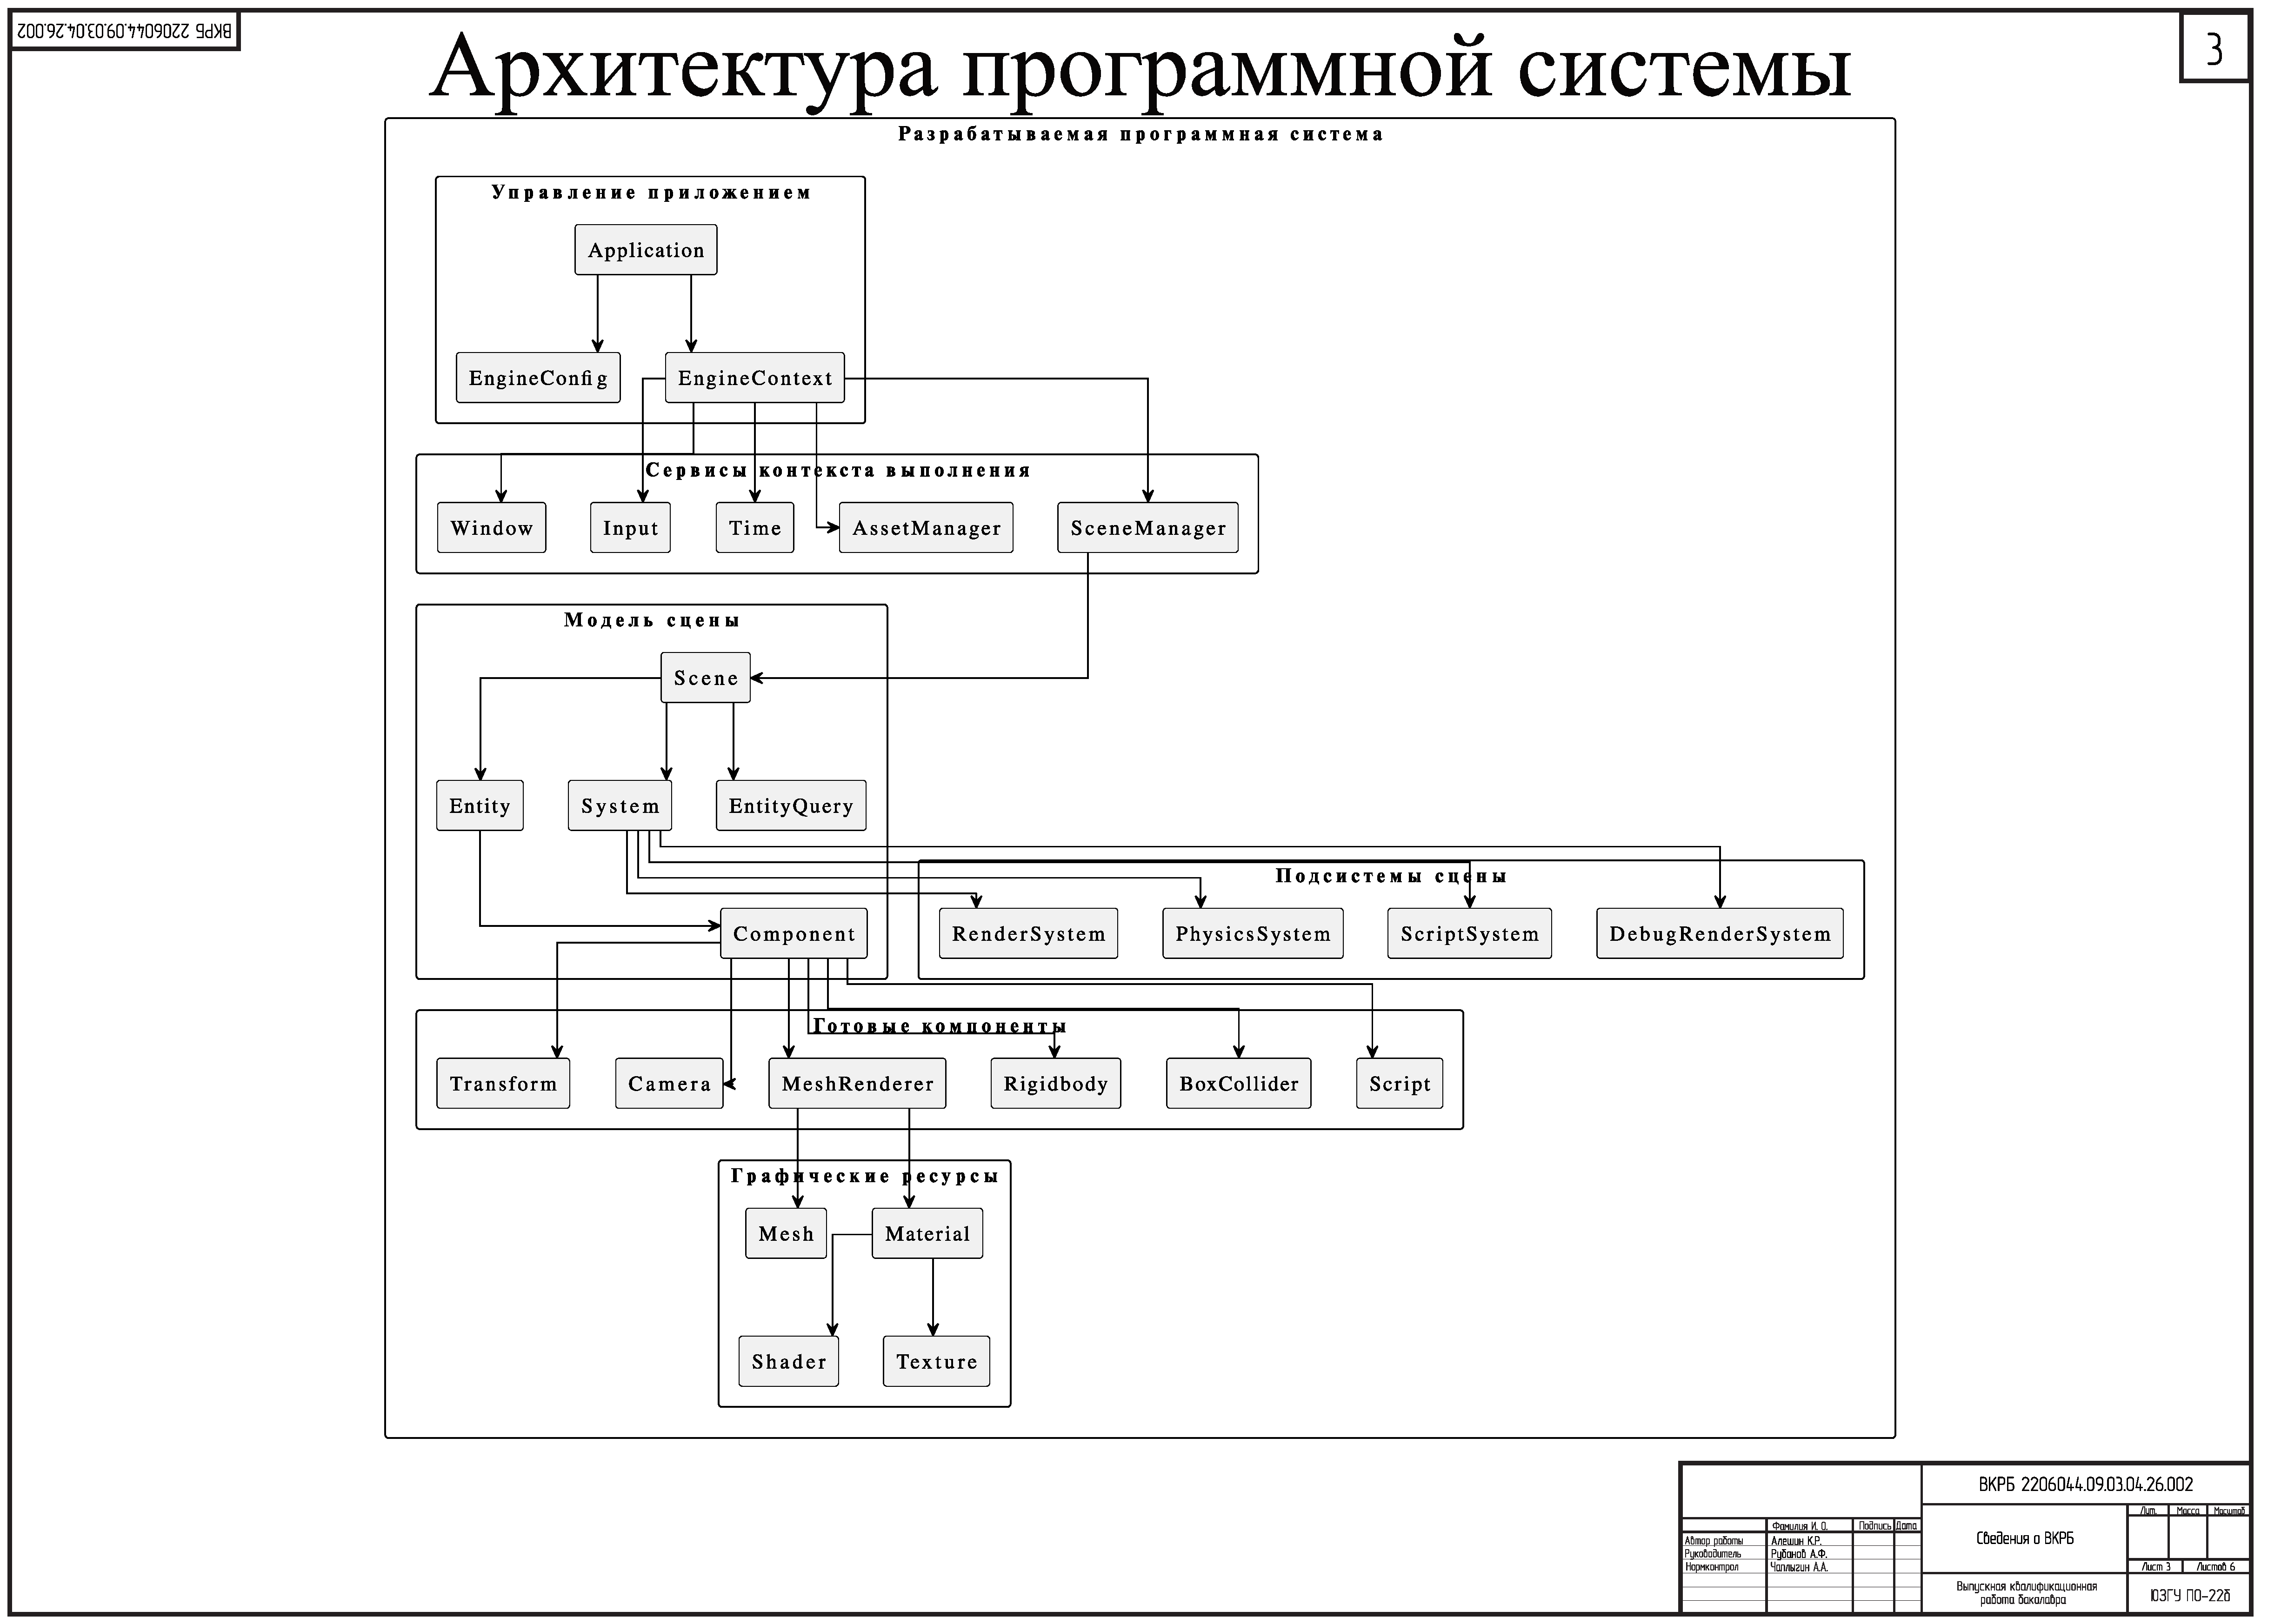
\includegraphics[width=0.82\linewidth]{posters/3.eps}
    \заголовок{Архитектура программной системы}
    \label{pl3:image}
\end{плакат}

\begin{плакат}
    
\includegraphics[width=0.82\linewidth]{posters/4.eps}
    \заголовок{Компонентная модель программной системы}
    \label{pl4:image}
\end{плакат}

\begin{плакат}
    
\includegraphics[width=0.82\linewidth]{posters/5.eps}
    \заголовок{Жизненный цикл кадра приложения}
    \label{pl5:image}
\end{плакат}

\begin{плакат}
    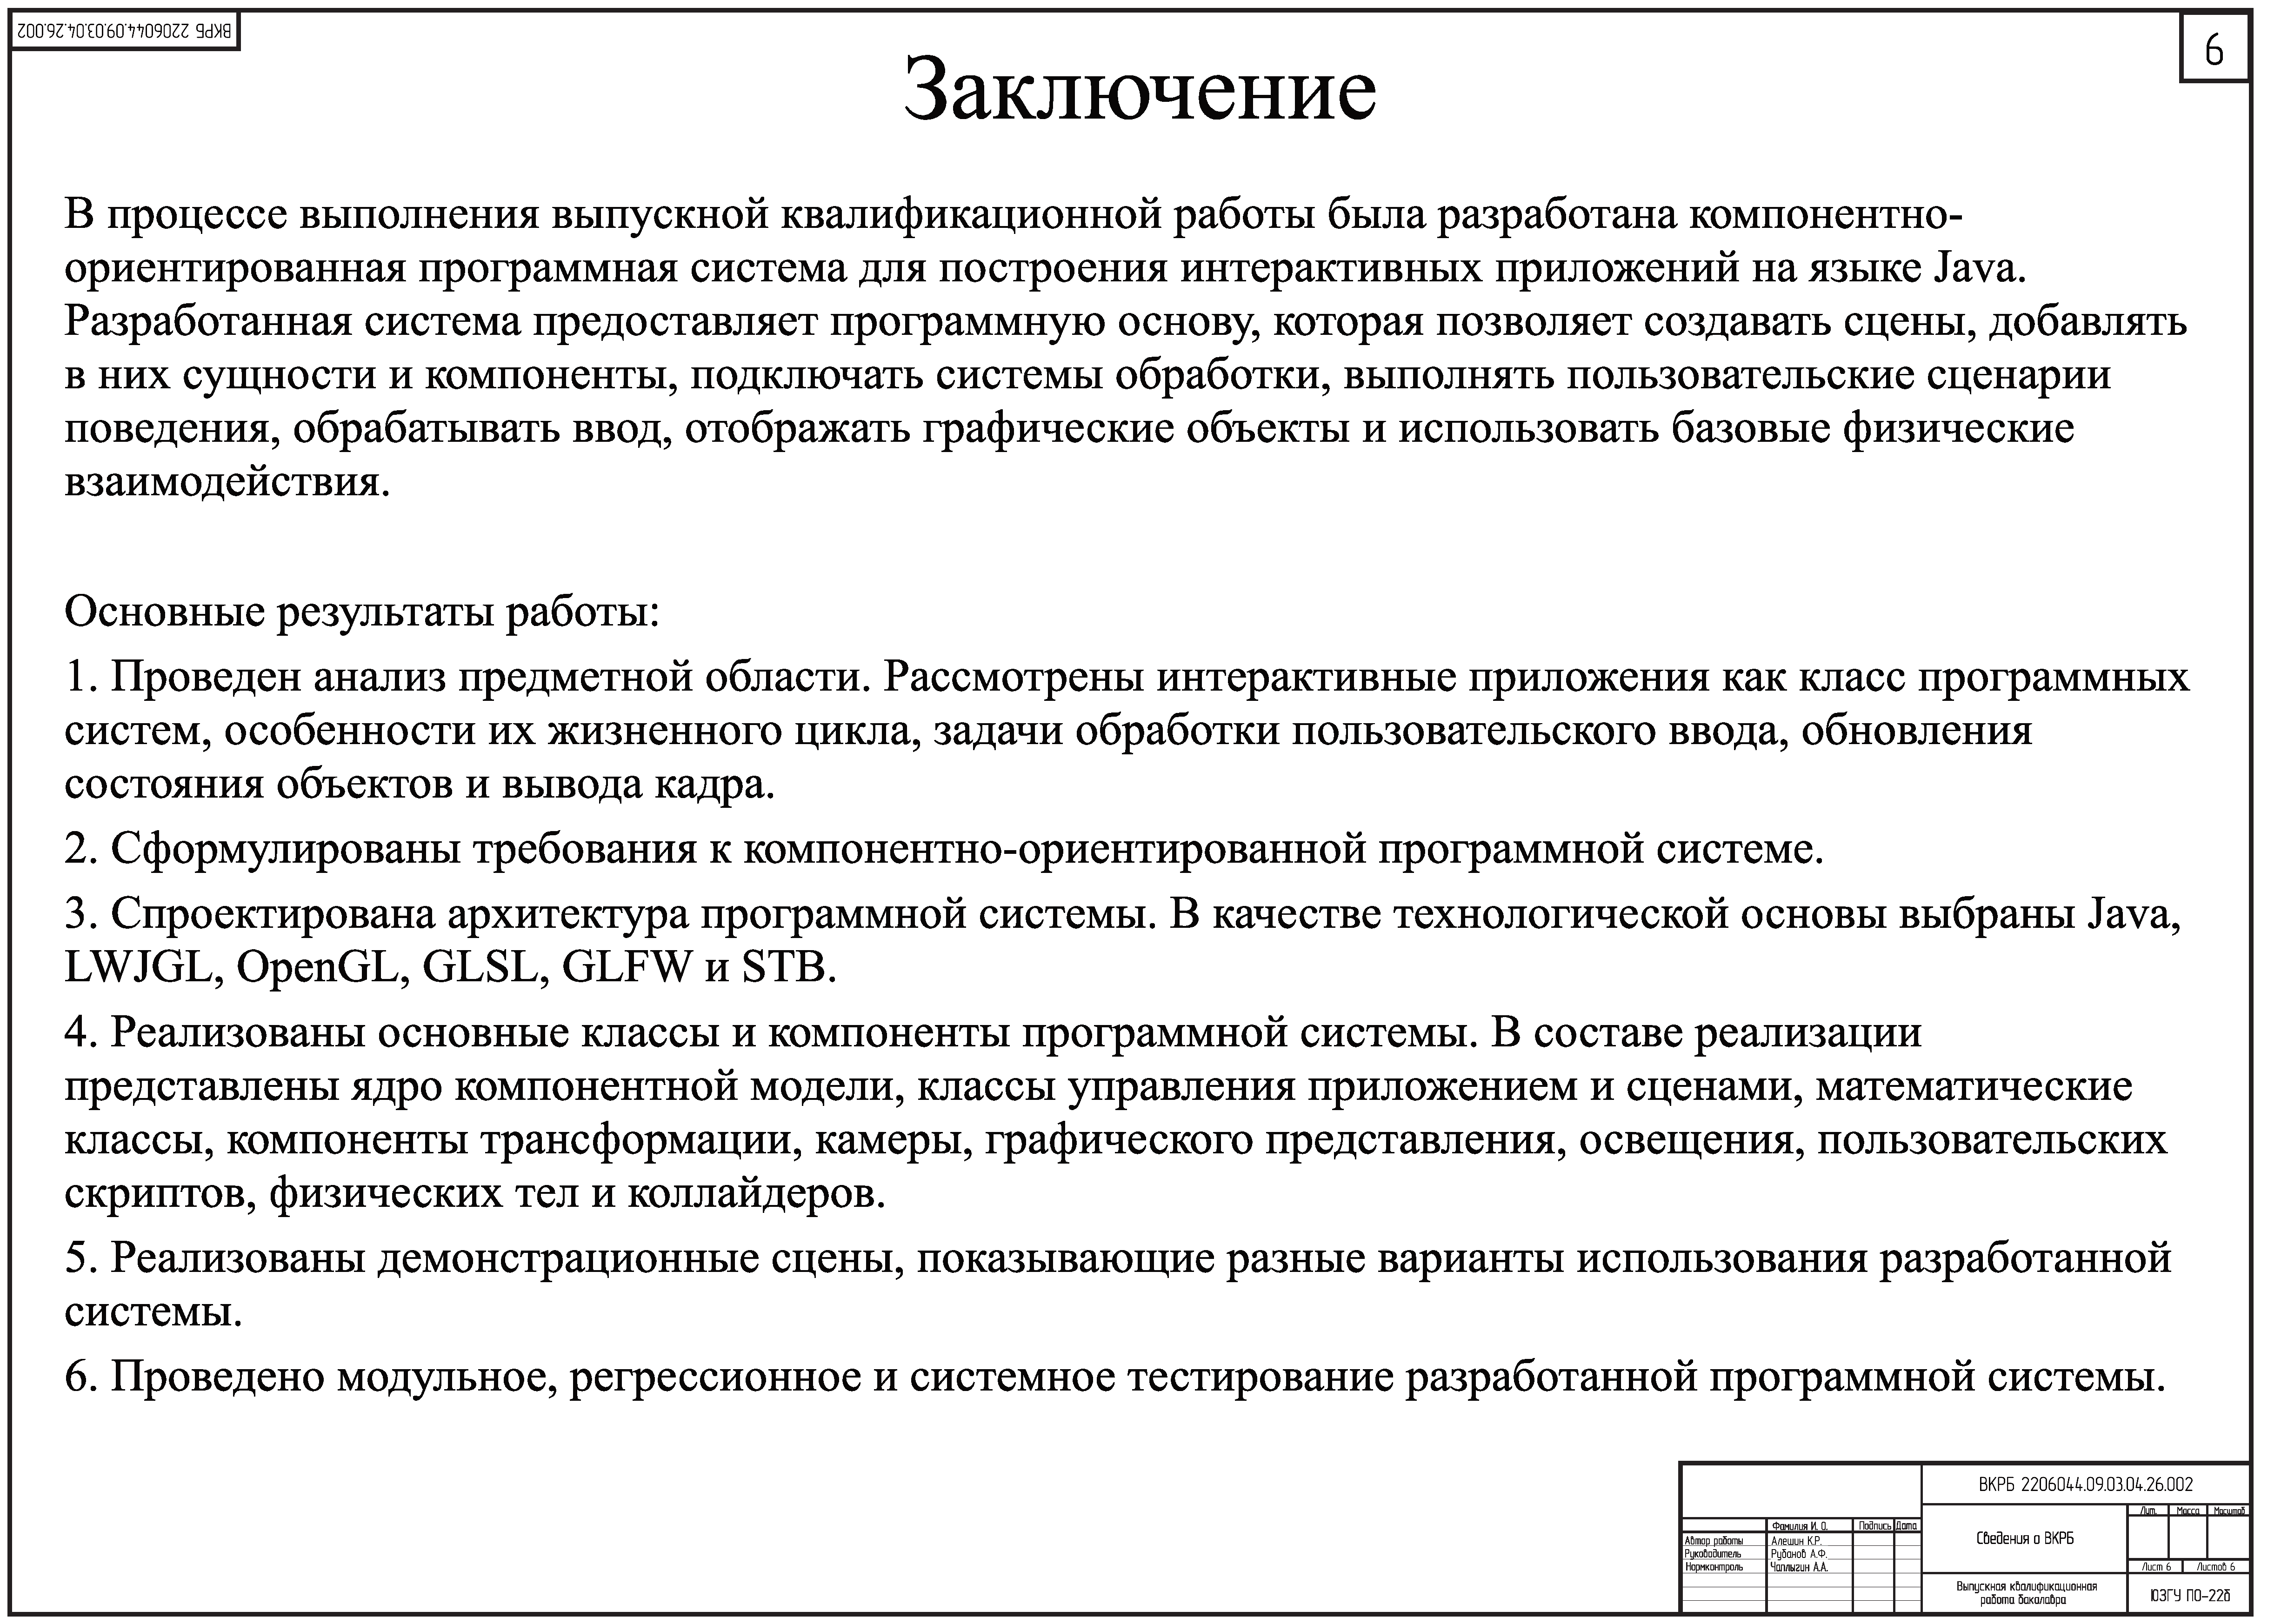
\includegraphics[width=0.82\linewidth]{posters/6.eps}
    \заголовок{Результаты разработки и тестирования}
    \label{pl6:image}
\end{плакат}

\end{landscape}
